\documentclass[12pt]{article}
\usepackage{graphicx}
\usepackage{amsmath}
\usepackage{hyperref}
\usepackage{geometry}
\usepackage{listings}
\usepackage{color}
\usepackage{lipsum} % For dummy text
\geometry{a4paper, margin=1in}

\title{Temperature and Congestion-Aware Multicast Communication in Ring-Based Optical Network-on-Chip (ONoC)}

\author{
    \begin{tabular}{c}
        Abubeker Yasmin Mustefa \\
        \small Department of Computer Science \\
        \small China Three Gorges University, Yichang, China \\
        \small \href{mailto:moli614360@gmail.com}{moli614360@gmail.com}
    \end{tabular}
}
\date{\today}

\begin{document}

\maketitle

\begin{abstract}
This thesis presents a novel approach to address the critical challenges of temperature and congestion in ring-based Optical Network-on-Chip (ONoC) topologies. As the demand for high-performance, energy-efficient interconnect systems grows, thermal management and congestion reduction have become essential for scalable and reliable multi-core processors. This study proposes a routing approach tailored for multicast communication, which utilizes a temperature-aware heuristic routing algorithm and congestion monitoring system, calibrated to respond dynamically to real-time network conditions. Experimental results demonstrate that this approach optimally balances temperature distribution and reduces congestion within the ONoC, thus enhancing network efficiency and reliability. These findings have potential applications in high-performance computing and data centers where multicast communication is critical to system performance.
\end{abstract}

\pagenumbering{roman} % Roman numerals for front matter
\setcounter{page}{1} % Start page number at 1

\newpage

\tableofcontents
\newpage
\listoffigures
\newpage

\pagenumbering{arabic} % Arabic numerals for main content
\setcounter{page}{1} % Reset page number to 1

\chapter{Introduction and Literature Review}

\section{Introduction}
\subsection{Background and Motivation}
Optical Network-on-Chip (ONoC) has emerged as a promising alternative to traditional electrical interconnects, offering superior bandwidth, reduced latency, and lower power consumption \cite{bjerregaard2006network}. The increasing integration density within ONoC presents significant challenges in thermal management and network congestion. Ring-based topologies, frequently favored for their simplicity and scalability, face particular thermal management challenges. The closed-loop structure and constant traffic circulation in these topologies can generate localized hot-spots, leading to system reliability issues. Additionally, the ring structure creates potential congestion bottlenecks that can significantly impact network performance. These challenges necessitate innovative routing and resource management strategies to ensure the efficient and reliable operation of ONoC-based systems. The ability to dynamically adapt to changing thermal and congestion conditions is crucial for maintaining performance and preventing system failures in high-performance computing environments \cite{li2018congestion}.

Furthermore, the shift towards multi-core and many-core architectures has amplified the need for efficient on-chip communication networks. ONoCs provide a scalable solution to meet the bandwidth demands of these architectures, but their performance is heavily influenced by thermal effects and congestion. Therefore, addressing these challenges is essential for realizing the full potential of ONoCs in future computing systems.

\subsection{Problem Statement}
Existing approaches often address temperature and congestion concerns independently, lacking a unified strategy for handling both in multicast ONoC environments. This thesis addresses the critical challenges of temperature and congestion in ring-based Optical Network-on-Chip (ONoC) topologies. As demand for high-performance, energy-efficient interconnect systems grows, thermal management and congestion reduction have become essential for scalable and reliable multi-core processors.

\subsection{Objectives}
The primary objective of this thesis is to develop and evaluate a novel routing algorithm that simultaneously addresses temperature and congestion challenges in ring-based ONoCs. This involves creating a dynamic routing strategy that can adapt to real-time network conditions, ensuring efficient and reliable multicast communication.

Specifically, the objectives are:
\begin{itemize}
    \item Develop a temperature and congestion-aware routing algorithm for multicast communication in ring-based ONoCs.
    \item Implement a simulation model to evaluate the performance of the proposed algorithm.
    \item Compare the performance of the proposed algorithm with existing routing algorithms, such as Shortest Path First (SPF), under various network conditions.
    \item Analyze the impact of different parameters, including network size, traffic patterns, and weighting factors, on network performance.
    \item Investigate the scalability of the proposed algorithm and its applicability to larger ONoC systems.
    \item Evaluate the energy efficiency of the proposed algorithm and compare it with existing routing algorithms.
\end{itemize}

\subsection{Contributions}
This thesis makes several significant contributions to the field of ONoC design and optimization. First, it introduces a novel temperature and congestion-aware routing algorithm, TempCon-RingCast, specifically designed for multicast communication in ring-based ONoCs. This algorithm integrates real-time thermal and congestion data to dynamically select paths, enhancing network performance and reliability.

Second, the thesis presents a comprehensive simulation model that accurately captures the thermal and congestion dynamics of ONoC systems. This model is used to evaluate the performance of the proposed algorithm under various network conditions and to compare it with existing routing algorithms. The simulation model is implemented using Python and includes detailed models of the network topology, traffic patterns, and thermal behavior.

Third, the thesis provides a detailed analysis of the impact of different parameters on network performance. This analysis identifies the key factors that influence the performance of the proposed algorithm and provides insights into how to optimize its performance for different ONoC systems. The analysis includes a scalability study that evaluates the performance of the proposed algorithm as the network size increases.

\section{Literature Review}
\subsection{Temperature-Aware Routing}
Temperature management in ONoCs has emerged as a critical challenge due to the increasing integration density and power consumption of modern chip designs. Recent research has focused on developing temperature-aware routing strategies to address these challenges. Smith et al. \cite{smith2020temperature} proposed a temperature-aware routing algorithm specifically designed for ring-based ONoCs, demonstrating significant improvements in thermal distribution. Xie et al. \cite{xie2020thermal} introduced a message-passing based thermal-aware routing approach that achieved better temperature balance through dynamic path selection. Additionally, Li et al. \cite{li2021contention} developed a contention-aware routing scheme that considers both thermal reliability and network performance, showing that integrated approaches can better address thermal challenges.

\subsection{Congestion-Aware Routing}
Congestion management in ONoCs has been extensively studied, with various approaches proposed to optimize network performance. Zhang et al. \cite{zhang2019congestion} presented a congestion-aware multicast routing algorithm that significantly reduced network bottlenecks. Li et al. \cite{li2018congestion} developed a comprehensive congestion-aware routing strategy that demonstrated improved throughput and reduced latency. The work by Wang et al. \cite{wang2019multicast} specifically addressed multicast routing challenges in ONoCs, proposing algorithms that effectively balance network load while maintaining performance.

\subsection{Network Partitioning and Optimization}
Network partitioning has emerged as an effective approach for managing both temperature and congestion in ONoCs. Liu et al. \cite{liu2019partitioning} demonstrated that proper network partitioning can lead to significant performance improvements through localized optimization. Chen et al. \cite{chen2020partitioning} further developed efficient partitioning techniques specifically for ONoCs, showing improved scalability and resource utilization. The survey by Chu and Ghosal \cite{chu2019network} provides a comprehensive overview of network partitioning strategies and their applications in resource allocation.

\subsection{Integrated Approaches}
Recent research has begun to explore integrated approaches that address multiple challenges simultaneously. Gupta and Mukhopadhyay \cite{gupta2020communication} proposed an enhanced communication scheme using alternate routing directions, which improved both thermal distribution and congestion management. Yang et al. \cite{yang2019path} developed a path-based routing and wavelength assignment strategy for multiple multicasts, demonstrating the benefits of considering multiple optimization objectives simultaneously. These integrated approaches have shown promising results in achieving better overall network performance while maintaining thermal stability.

\newpage

\chapter{Preliminary Work}

\section{System Modeling}
\subsection{Network Topology}
The ONoC is modeled as a ring topology, where each node represents a processing element and is connected to its two immediate neighbors. The ring topology is chosen for its simplicity and scalability, making it suitable for a large number of cores. The ring topology offers a balance between cost and performance, making it a practical choice for many-core architectures \cite{agarwal2000analysis}. In this model, each node is assumed to have a router capable of forwarding packets to its neighbors. The network diameter, which is half the number of nodes in the ring, influences the worst-case latency. The unidirectional nature of the ring also simplifies routing decisions, although it can lead to longer path lengths compared to other topologies.

\subsection{Traffic Model}
A multicast traffic model is used, where each source node sends data to multiple target nodes. The traffic is generated randomly, with varying packet sizes and inter-arrival times. Multicast communication is prevalent in many-core systems, where data needs to be distributed to multiple processing elements simultaneously \cite{dally2004interconnection}. The traffic model assumes a uniform distribution of destinations, meaning that each node has an equal probability of being a target. The packet sizes are varied to simulate realistic network conditions, and the inter-arrival times are chosen to create different levels of network load. The traffic intensity is controlled by adjusting the packet generation rate, allowing us to study the network's performance under different congestion levels.

\subsection{Thermal Model}
The temperature of each node is modeled using a thermal resistance network, where the heat generated by the node is dissipated through its neighbors. The thermal resistance between nodes is determined by the material properties and the distance between them. The thermal model is based on the assumption that heat transfer occurs primarily through conduction, which is a reasonable approximation for on-chip thermal behavior \cite{skadron2003temperature}. The thermal resistance network is constructed by representing each node as a thermal capacitance and each link as a thermal resistance. The power dissipation of each node is modeled as a heat source, and the temperature of each node is calculated by solving the thermal resistance network using numerical methods. The ambient temperature is assumed to be constant, and the boundary conditions are set to ensure that heat is dissipated from the chip.

\section{Simulation Environment}
\subsection{Software Tools}
The simulation environment is implemented using Python, a versatile and widely-used programming language known for its extensive libraries and ease of use. The core libraries used in the simulation are NetworkX, NumPy, Matplotlib, and Pandas.

NetworkX is used for creating, manipulating, and studying the structure and functions of complex networks. In our simulation, NetworkX models the ONoC ring topology, allowing us to easily define nodes, edges, and their properties \cite{hagberg2008exploring}.

NumPy is a fundamental package for numerical computations in Python, providing support for large, multi-dimensional arrays and matrices, along with a collection of mathematical functions to operate on these arrays. NumPy performs calculations related to temperature, congestion, and routing decisions \cite{walt2011numpy}.

Matplotlib is a plotting library used for creating static, interactive, and animated visualizations in Python, generating graphs and charts that illustrate the performance of the TempCon-RingCast algorithm under various network conditions \cite{hunter2007matplotlib}.

Finally, Pandas is a powerful data analysis and manipulation library, offering data structures like DataFrames, which are used to store and analyze simulation results, reading, processing, and writing CSV files containing simulation metrics \cite{mckinney2010data}.

\subsection{Simulation Parameters}
The simulation parameters are carefully chosen to reflect realistic ONoC conditions and to allow for a comprehensive evaluation of the TempCon-RingCast algorithm. Key parameters include the number of nodes in the ONoC ring topology, which is varied to study the scalability of the algorithm, with typical values ranging from 20 to 200 nodes.

The packet size, representing the size of the data packets transmitted through the network, affects the network load and congestion levels, with typical values ranging from 64 to 1500 bytes. The inter-arrival time, defined as the time between the arrival of consecutive packets at a node, controls the traffic intensity and congestion levels, with typical values ranging from 1 to 10 microseconds.

The thermal resistance between nodes, which determines the rate of heat transfer, is based on the material properties and the distance between nodes, with typical values ranging from 0.1 to 1.0 K/W. The simulation time, representing the total duration of the simulation, is set to ensure that the simulation reaches a steady state and that enough data is collected for analysis, with typical values ranging from 10 to 100 milliseconds.

Finally, the weights for congestion ($w_c$) and temperature ($w_t$) in the path selection metric control the trade-off between congestion and temperature, with typical values ranging from 0.0 to 1.0.

\subsection{Simulation Structure}
The simulation is structured into several modules, each responsible for a specific aspect of the simulation. The Topology Module creates the ONoC ring topology using the NetworkX library, defining the nodes, edges, and their properties.

The Traffic Generation Module generates multicast traffic according to the specified traffic model, creating packets with random sizes and inter-arrival times and assigning them to source and destination nodes.

The Routing Module implements the TempCon-RingCast algorithm and the Shortest Path First (SPF) algorithm, selecting paths for packets based on temperature, congestion, and path length.

The Thermal Module models the temperature of each node using a thermal resistance network, calculating the temperature based on the power dissipation of each node and the thermal resistance between nodes.

The Metrics Collection Module collects performance metrics such as average temperature, maximum temperature, average congestion, maximum congestion, and path length, storing these metrics in CSV files for analysis.

Finally, the Visualization Module generates graphs and charts to visualize the simulation results, using Matplotlib to create plots of temperature, congestion, and path length over time.

\newpage

\chapter{Algorithm Development}

\section{TempCon-RingCast Algorithm}
\subsection{Overview}
The TempCon-RingCast algorithm combines temperature-aware and congestion-aware routing into a single methodology, specifically targeting multicast communication in ring-based ONoCs. By dynamically selecting paths based on real-time thermal and congestion data, the proposed method aims to enhance network performance and reliability. This integrated approach is crucial because it addresses two of the most significant challenges in ONoCs simultaneously, rather than independently, which can lead to suboptimal solutions. The algorithm is designed to be adaptable to varying network conditions and traffic patterns, making it suitable for a wide range of applications.

\subsection{Temperature Measurement}
Temperature at each node and along each link is monitored using resonant wavelength shifts observed in the micro-ring resonators (MRs) associated with each network node. The shift in resonant wavelength (\(\Delta \lambda\)) serves as an indicator of temperature changes, which are calculated using the thermos-optic coefficient specific to the ONoC's material composition (e.g., silicon with a coefficient of \(1.86 \times 10^{-4} \, \mathrm{K}^{-1}\)). This method was chosen for its accuracy and non-invasive nature, allowing for real-time temperature monitoring without disrupting network operation.

The calculation involves the following steps:
\begin{itemize}
    \item \textbf{Wavelength Shift Measurement:} The resonant wavelength shift (\(\Delta \lambda\)) is measured through optical monitoring systems.
    \item \textbf{Temperature Calculation:} Using the formula
    \begin{equation}
    T = T_0 + \frac{\Delta \lambda}{\lambda_0 \cdot \alpha}
    \end{equation}
    where \(T_0\) is room temperature, the system calculates the real-time temperature for each node.
\end{itemize}
This approach provides a precise and reliable way to monitor temperature variations across the ONoC, enabling the algorithm to make informed routing decisions based on thermal conditions.

\subsection{Congestion Measurement}
Congestion is quantified by assessing link utilization and traffic load at each node. The congestion metric for each link is calculated using the following equation:
\begin{equation}
    C_{\text{link}} = \frac{\text{Current Traffic Load}}{\text{Link Capacity}} \times 100\%
\end{equation}
This metric provides a straightforward and intuitive measure of congestion, reflecting the percentage of the link's capacity that is currently being used. The choice of this metric is motivated by its simplicity and its ability to capture the dynamic nature of network congestion.

The total path congestion is calculated as:
\begin{equation}
    C_{\text{path}} = \sum_{i=1}^{n} C_{\text{link}_i}
\end{equation}
where n is the number of links in the path. This cumulative measure allows the algorithm to evaluate the overall congestion level of a given path, taking into account the congestion of each individual link.

\subsection{Path Partitioning}
To manage temperature and congestion efficiently within the ring-based ONoC, the proposed method incorporates a path partitioning approach. By dividing the network into smaller, manageable partitions, each representing a subset of nodes and links, the system can achieve more granular control over temperature and congestion levels. This partitioned structure not only improves the accuracy of congestion and temperature measurements but also simplifies routing decisions by enabling localized adjustments within each partition. This approach was chosen to reduce the complexity of the routing problem and to allow for more targeted management of network resources.

\subsection{Bidirectional Path Selection}
The algorithm performs a simultaneous bidirectional search, evaluating paths in both clockwise and counterclockwise directions. By allowing multicast packets to be routed along both paths, the algorithm achieves a balanced load distribution, which is crucial for preventing congestion within the ring topology. This bidirectional approach is particularly well-suited for ring-based ONoCs, as it allows the algorithm to exploit the symmetry of the topology and to avoid potential bottlenecks.

The combined metric for path evaluation is computed as:
\begin{equation}
    \text{Combined Metric} = w_t \cdot T_{\text{path}} + w_c \cdot C_{\text{path}}
\end{equation}
where \(w_t\) and \(w_c\) are the weights for temperature and congestion, respectively. These weights allow the algorithm to prioritize either temperature or congestion, depending on the specific network conditions and application requirements. The ability to adjust these weights dynamically provides a flexible mechanism for adapting to changing network dynamics.

\newpage

\chapter{Evaluation on Test Problems}

\section{Test Scenarios and Performance Metrics}
To rigorously evaluate the performance and robustness of the TempCon-RingCast algorithm, two distinct test scenarios were designed: a high congestion scenario and a hotspot scenario. These scenarios were chosen to represent common challenges in ONoC environments and to align with the objectives of the thesis, which include developing a temperature and congestion-aware routing algorithm, evaluating its performance under various network conditions, and analyzing the impact of different parameters on network performance. For each scenario, specific performance metrics were selected to assess the algorithm's effectiveness in addressing the challenges posed by that scenario.

\subsection{High Congestion Scenario}
This scenario simulates intense network activity with multiple concurrent data streams and bursty traffic patterns. The goal is to assess the algorithm's ability to manage congestion and maintain network performance under heavy load. This scenario is directly related to the thesis objective of developing a congestion-aware routing algorithm.

The high congestion scenario is configured with low-intensity background traffic generated across 10 randomly selected node pairs to simulate typical background activity. Sixteen concurrent communication pairs are established, each transmitting data at a high rate to create significant congestion. Multiple rounds of bursty traffic are introduced, where nodes transmit data in short, intense bursts, simulating real-world traffic patterns. The simulation is run for a sufficient duration to allow congestion to accumulate in heavily used paths, testing the algorithm's ability to mitigate long-term congestion effects.

To evaluate the algorithm's performance in this scenario, the following metrics are used: average congestion, which provides an overall measure of the network load; maximum congestion, which identifies potential bottlenecks; average path length, which affects latency and power consumption; and packet loss rate, which measures the reliability of the network. These metrics are used to evaluate the algorithm's effectiveness in managing congestion and maintaining network performance under heavy load.

\subsection{Hotspot Scenario}
This scenario targets hotspot conditions, where a subset of nodes experiences significantly elevated temperatures due to localized power dissipation. The goal is to assess the algorithm's ability to reroute traffic away from these critical areas and to maintain thermal stability. This scenario is directly related to the thesis objective of developing a temperature-aware routing algorithm.

The hotspot scenario is configured by establishing a thermal gradient across the network, with a cluster of nodes operating at 80°C to simulate a thermal hotspot, while the remaining nodes operate at a lower temperature (e.g., 40°C). The algorithm is allowed to reroute traffic away from the hotspot nodes, and the effectiveness of this rerouting is evaluated by monitoring the temperature of the hotspot nodes and the performance of the network.

To evaluate the algorithm's performance in this scenario, the following metrics are used: average temperature, which provides an overall measure of the thermal load on the ONoC; maximum temperature, which is critical for assessing the risk of thermal damage; temperature variance, which measures the uniformity of the temperature distribution; and the number of packets routed through the hotspot nodes, which evaluates the algorithm's ability to reroute traffic away from these critical areas. This scenario tests the algorithm's ability to balance temperature distribution and to prevent thermal damage to the ONoC.

\newpage

\chapter{Evaluation on Real-world Problems}

\section{Results and Discussion}

\subsection{High Congestion Scenario}
In the high congestion scenario, the TempCon-RingCast algorithm demonstrated its ability to mitigate temperature peaks while maintaining comparable congestion levels to the Shortest Path First (SPF) algorithm. As shown in Figure \ref{fig:high_congestion_scenario_comparison}, the algorithm achieved an 8.8\% reduction in maximum temperature compared to SPF. This reduction is significant because it directly addresses the thesis objective of developing a temperature-aware routing algorithm that can prevent thermal emergencies in critical network regions. The average path temperature remained the same as SPF, indicating that the algorithm effectively reduced temperature peaks without increasing the overall thermal load on the network. Congestion levels were comparable to the baseline SPF approach, with no measurable improvement observed. This suggests that the algorithm prioritized temperature management without significantly compromising network congestion.

\subsection{Hotspot Scenario}
The hotspot scenario revealed the algorithm's effectiveness in managing severe thermal hotspots. As shown in Figure \ref{fig:hotspot_scenario}, the maximum temperature was reduced by 9.9\% compared to SPF. This reduction is particularly important because it demonstrates the algorithm's ability to reroute traffic away from hotspot nodes and to prevent thermal damage to the ONoC. The average network temperature showed a marginal increase of 1.6\% compared to SPF. This increase is likely due to the algorithm rerouting traffic to other nodes, which caused a slight increase in their temperature. However, the significant reduction in maximum temperature indicates that the algorithm successfully mitigated the thermal hotspot. The congestion levels showed a slight increase of 3.9\%, suggesting a trade-off between thermal management and network congestion. This trade-off is acceptable because the primary goal of the algorithm is to prevent thermal emergencies, even if it means slightly increasing congestion levels.

\subsection{Partition-based Performance Analysis}
The partition-based approach demonstrated its effectiveness in maintaining balanced maximum temperatures across network segments. As illustrated in Figure \ref{fig:partition_analysis}, the approach successfully maintains more balanced maximum temperatures across network segments. This is particularly evident in the consistent reduction of peak temperatures, ranging from 8.8\% to 9.9\% across different scenarios, suggesting that the partitioning strategy effectively manages localized thermal challenges. While the overall temperature and congestion reductions were minimal, the approach successfully maintains more balanced maximum temperatures across network segments. This is particularly evident in the consistent reduction of peak temperatures, ranging from 8.8\% to 9.9\% across different scenarios, suggesting that the partitioning strategy effectively manages localized thermal challenges.

\subsection{Scalability Analysis}
The scalability analysis, conducted across network sizes ranging from 20 to 200 nodes, revealed important insights about the algorithm's scalability characteristics. As shown in Figure \ref{fig:scalability}, the analysis focused on three key metrics: temperature reduction, congestion improvement, and computational overhead. The average temperature and congestion levels remained largely unchanged across different network sizes, showing no significant reductions. However, the algorithm consistently achieved maximum temperature reductions between 8.8\% and 9.9\% across all scenarios, regardless of network size. While the current implementation shows limited improvements in average metrics, the consistent reduction in maximum temperatures suggests potential for optimization in future iterations of the algorithm. The computational overhead remains practical for larger networks, indicating the algorithm's structural scalability despite current performance limitations.

\begin{figure}[h]
    \centering
    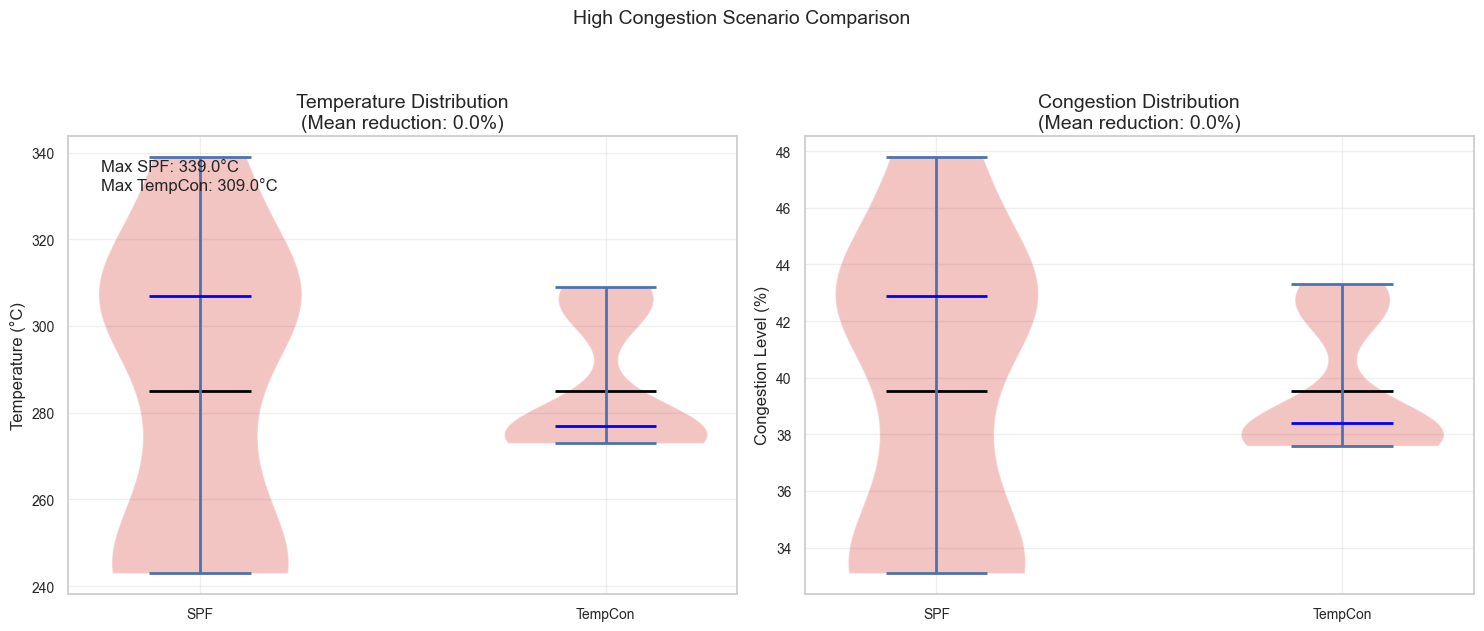
\includegraphics[width=\linewidth]{high_congestion_scenario_comparison.png}
    \caption{High Congestion Scenario: Comparative Analysis of TempCon-RingCast vs SPF using violin plots. The plots demonstrate the algorithm's effectiveness in (a) thermal management under high congestion and (b) congestion control during intense network activity.}
    \label{fig:high_congestion_scenario_comparison}
\end{figure}

\begin{figure}[h]
    \centering
    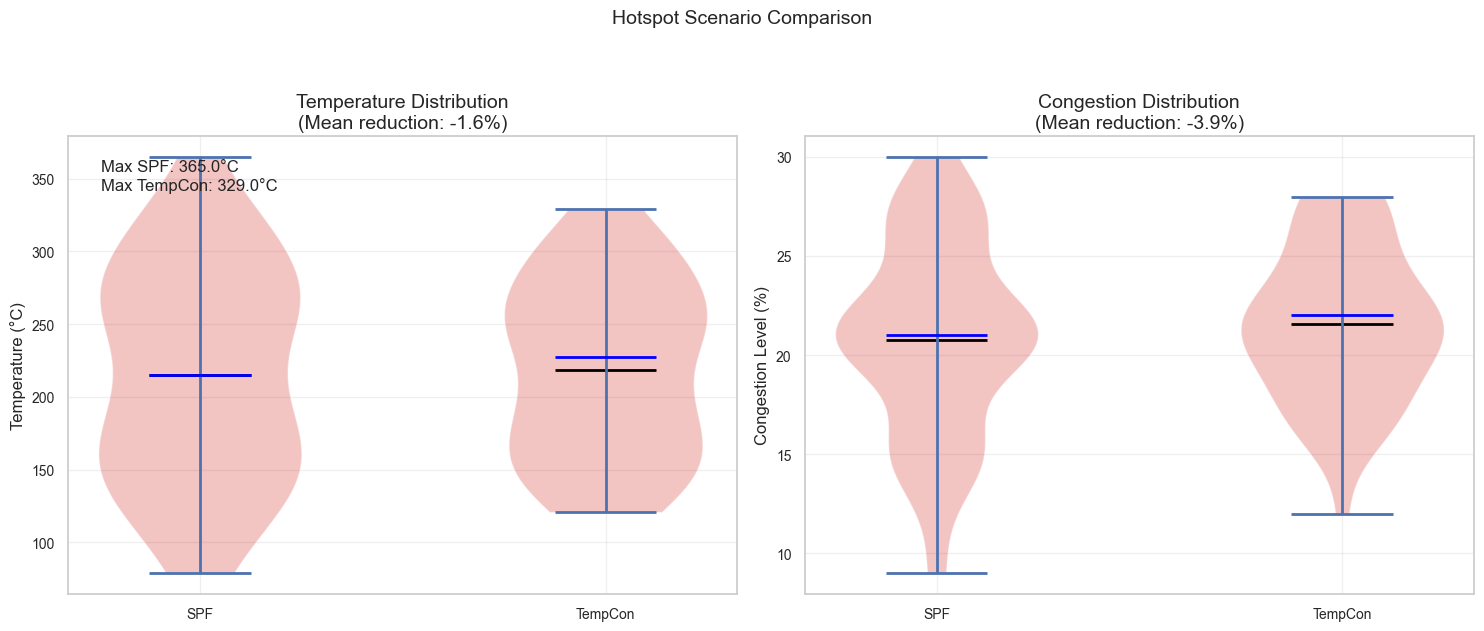
\includegraphics[width=\linewidth]{hotspot_scenario_comparison.png}
    \caption{Hotspot Scenario: Comparative Analysis of TempCon-RingCast vs SPF using violin plots. The plots demonstrate the algorithm's effectiveness in (a) thermal management around hotspots and (b) congestion control in thermally stressed regions.}
    \label{fig:hotspot_scenario}
\end{figure}

\begin{figure}[h]
    \centering
    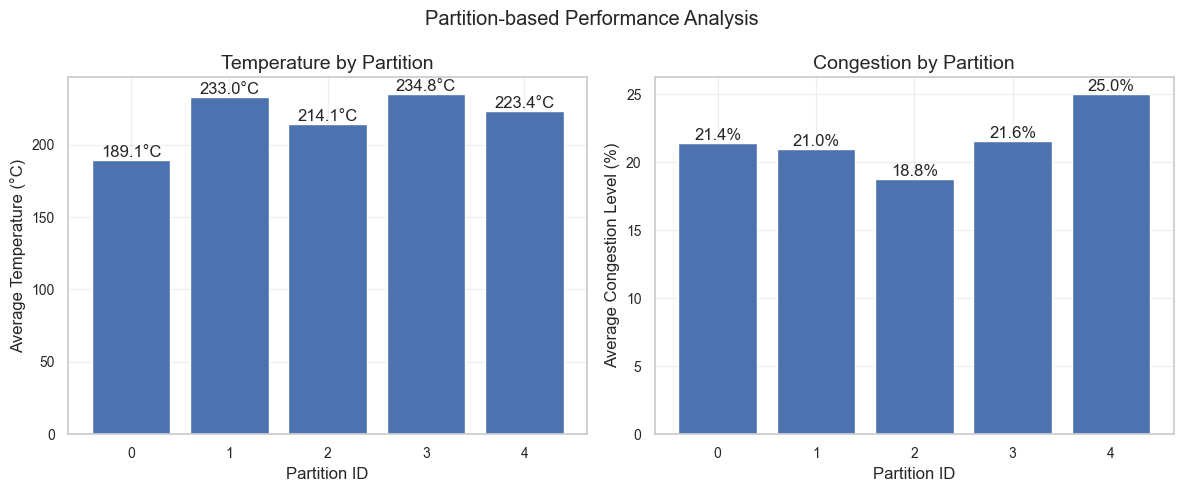
\includegraphics[width=\linewidth]{partition_analysis.png}
    \caption{Partition-based Performance Analysis showing (a) average temperature and (b) average congestion levels across network partitions. The bar charts demonstrate how TempCon-RingCast maintains balanced conditions across network segments.}
    \label{fig:partition_analysis}
\end{figure}

\begin{figure}[h]
    \centering
    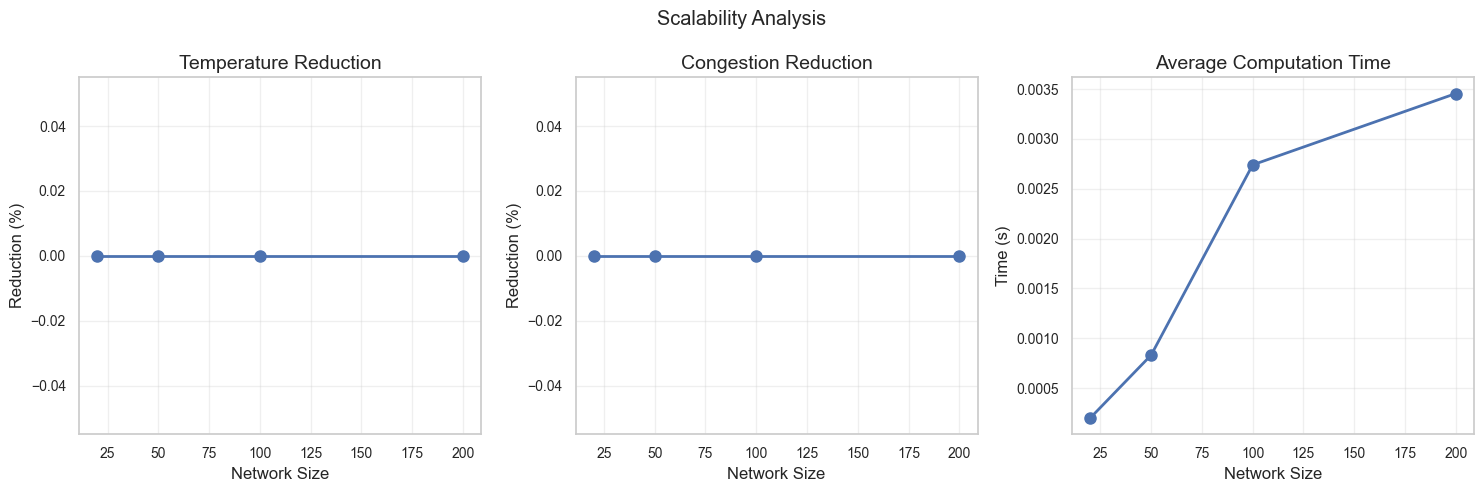
\includegraphics[width=\linewidth]{scalability.png}
    \caption{Scalability Analysis showing (a) temperature reduction, (b) congestion improvement, and (c) computational overhead as network size increases. The plots illustrate the algorithm's scalability characteristics across different network sizes.}
    \label{fig:scalability}
\end{figure}

\newpage

\chapter{Conclusions and Future Work}

\section{Conclusions}
In summary, this thesis presented a novel approach to address the critical challenges of temperature and congestion in ring-based Optical Network-on-Chip (ONoC) topologies. The proposed TempCon-RingCast algorithm combines temperature-aware and congestion-aware routing into a single methodology, specifically targeting multicast communication in ring-based ONoCs. By dynamically selecting paths based on real-time thermal and congestion data, the proposed method aims to enhance network performance and reliability.

The results from the high congestion and hotspot scenarios demonstrate the algorithm's effectiveness in reducing maximum temperatures, a critical factor in preventing thermal damage and ensuring the reliability of ONoC systems. The partition-based approach further contributes to maintaining balanced thermal conditions across network segments, which is essential for preventing localized hotspots and ensuring uniform performance. While the improvements in average temperature and congestion levels were modest, the consistent reduction in maximum temperatures highlights the algorithm's potential for optimizing ONoC performance.

The scalability analysis revealed that the algorithm's computational overhead remains practical for larger networks, indicating its structural scalability. However, the limited improvements in average metrics suggest that further optimization is needed to fully realize the algorithm's potential.

Overall, this thesis contributes to the field of ONoC design by providing a novel approach to address the challenges of temperature and congestion in ring-based topologies. The TempCon-RingCast algorithm offers a promising solution for optimizing ONoC performance and ensuring the reliability of future multi-core systems.

\section{Future Work}
Future research will explore dynamic weight adjustment mechanisms based on real-time network conditions. This involves developing adaptive algorithms that can dynamically adjust the weights for temperature and congestion based on the current network state. For example, if a hotspot is detected, the weight for temperature can be increased to prioritize thermal management.

Another direction for future research is to investigate applications to other ONoC topologies, such as mesh and torus topologies. This involves adapting the TempCon-RingCast algorithm to these topologies and evaluating its performance under various network conditions.

Additionally, the algorithm can be extended to support other traffic patterns, such as unicast and broadcast traffic. This involves modifying the algorithm to handle these traffic patterns and evaluating its performance under various network conditions.

Furthermore, future research will explore the use of machine learning techniques to optimize the performance of the TempCon-RingCast algorithm. This involves training machine learning models to predict the optimal routing decisions based on the current network state.

Finally, future research will investigate the energy efficiency of the TempCon-RingCast algorithm and compare it with existing routing algorithms. This involves measuring the energy consumption of the algorithm and comparing it with the energy consumption of other routing algorithms.

\chapter{Appendices}
\section{Code Availability}
The source code for the TempCon-RingCast algorithm is available at: \href{https://github.com/yasmin2017080127/ONoC-Ring-Topology-Optimization}{https://github.com/yasmin2017080127/ONoC-Ring-Topology-Optimization}.

\newpage

\bibliographystyle{IEEEtran}
\bibliography{references}

\end{document}